\chapter{Description and Work Done}

As mentioned in chapter \ref{Introduction}, TarPy is a multi-agent platform that acts as the bridge between Tartarus and Python. Tartarus has it's core components written in SWI-Prolog, and the benefit of changing code on the fly, thus providing a dynamic nature to the code, is not available in modern programming languages. To preserve this critical aspect of Tartarus, SWI-Prolog must be the software's core language of operations. However, since we need to ease the syntax, statistically, the most suitable language is Python. Thus, the entire package is Python at the user's end and SWI-Prolog at the agent's end.

\section{Components}
There are many components present in files that may not be independent of each other in the interaction. Typically, we require specific files to be present in order to perform our required tasks. The following section would describe various typical components for our interaction. Note that the files can be more as per use case and need not have the same name as described in the subsections.

\subsection{Tartarus Prolog Platform}
First and foremost, we require the Tartarus platform file, which is written originally in Prolog. This file contains all the Tartarus predicates for our multi-agent platform. Thus, this file would act as a base file and function at the core of the entire Python - SWI-Prolog interaction system.

\subsection{PySwip}
 We need a way to execute Prolog queries via Python. A Python library called PySwip fulfills this requirement. PySwip is a Python - SWI-Prolog bridge enabling to query SWI-Prolog in Python programs. It features an (incomplete) SWI-Prolog foreign language interface, a utility class that makes it easy querying with Prolog, and a Pythonic interface. Once PySwip is imported into Python, access the Prolog module, and assign it to a Python object. The query object would make all the further queries to Prolog.

\subsection{Tartarus Python Wrapper}
Once we have a way to communicate and query Prolog via Python, we now focus on how this can be utilized for our purpose. Tartarus is present in a Prolog file. However, we aim to have Python constructs which we can use for our Python platforms running over Tartarus. Thus, we create a Python file called \textit{`Tartarus.py'} that contains functions that query the appropriate Prolog predicates by passing the necessary parameters.

\subsection{Python Handler}
Another one of Tartarus' prominent features is the mobility of agents. Agents can move from one platform to another, unlike other software that communicates information via message passing or other means. Tartarus agents, along with their mobility, can also carry information with them in the form of payloads, which are nothing but Prolog predicates.
\par For an agent, it is essential to define its behavior and goals. Thus, we add a handler along with the agent, which takes care of the requirement. However, the agent understands the handler written in Prolog, but the developer can define the handler more conveniently in Python. Thus, the user is supposed to write a handler file in Python. This handler file written in Python is added as a payload to the mobile agent via a function \textit{`add handler()'} defined in our \textit{`Tartarus.py'} file.

\subsection{Prolog Handler} \label{Prolog Handler}
Although the user in Python well defines the agent handler, it is inevitable to have a handler in Prolog, which would work at the core of agent control. The Prolog handler typically performs the following tasks:
\begin{itemize}
    \item Retrieving the Python handler and agent database from the payload.
    \item Writing the agent Python handler and database to appropriate files.
    \item Execute the Python handler as a process.
    \item Retrieve the modified agent database information into the agent payload.
    \item Delete the agent Python files written by Prolog handler.
    \item Perform any additional specified actions.
\end{itemize}

\subsection{Temporary Agent Files}
As mentioned in \ref{Prolog Handler}, the typical Prolog handler writes the agent Python handler and Database into appropriate files. Technically, these files are strings attached as payloads to the agent in the form of predicates. Since the file names need to be unique to every agent and decided by the Prolog handler, the typical file syntax followed for Naming these files are ``agentname\_\{TYPE\}.py" where agentname would be replaced by the name of the agent and TYPE can be anything from the set \{Database, handler\_Rec, ConvertData\_to\_string\}. The purposes of these files are as follows:
\begin{itemize}
    \item \textbf{agentname\_handler\_Rec.py} file is used to write the Python handler written by the user. Since handler is Python, to execute the information and make changes in the database, it is necessary to make a process to execute Python handler.
    \item \textbf{agentname\_Database.py} file stores all the relevant data about the agent.
    \item \textbf{agentname\_ConvertData\_to\_string.py} file is used to update the Database present in agent's payload predicate.
\end{itemize}

\section{Working}
\begin{figure}[!ht]
    \centerline{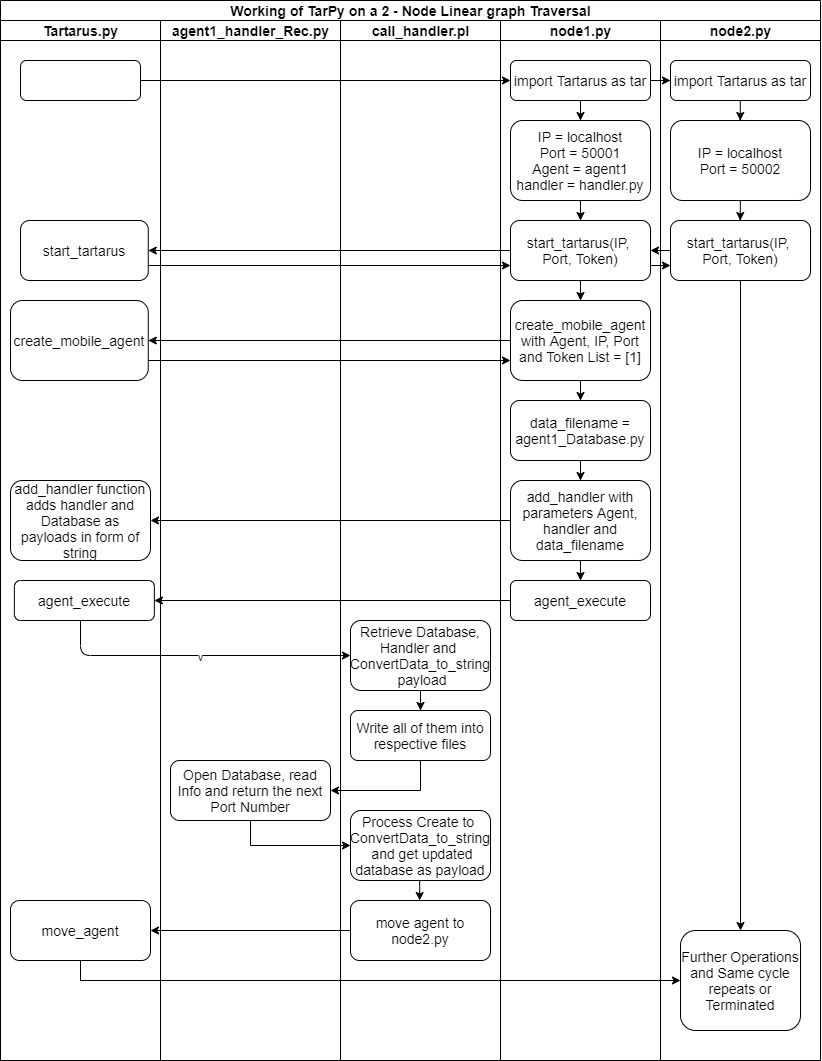
\includegraphics[width=\linewidth]{images/Working.jpg}}
    \caption{Working of TarPy for a 2 - Node Traversal}
    \label{working}
\end{figure}

Figure \ref{working} describes the working and interrelation of various components for a 2 - node traversal. \textit{node1.py} and \textit{node2.py} are the two node configuration files that execute different process instances on the same machine or another device. \textit{Tartarus.py} and \textit{platform.pl} (not shown in the figure) are present on every node. \text{handler.py} and \textit{agent1\_handler\_Rec.py} are the same programs, except that \textit{handler.py} is added as the initial payload while \textit{agent1\_handler\_Rec.py} is created by \textit{call\_handler.pl} for agent1. Thus \textit{handler.py} is not shown in the figure. The two temporary agent files, \textit{agent1\_Database.py} and \textit{agent1\_ConvertData\_to\_string.py}, are also created; however, their interaction is limited to \textit{agent1\_handler\_Rec.py}. Thus, these files are also not shown in the interaction.
\par Thus, the working of TarPy in this scenario can be described as follows:
\begin{enumerate}
    \item \textit{Tartarus.py} is imported into Python programs as `tar' in \textit{node1.py} and \textit{node2.py} 
    \item \textit{node1.py} decides IP as ``localhost" and Port as 50001 and \textit{node2.py} decide the same IP and Port as 50002.
    \item Both the nodes start the Tartarus instances by calling \textit{tar.start\_tartarus(IP, Port, 1)}, where 1 is a token for the platforms. It is necessary that node2 starts before node1 sends an agent.
\item node1 creates agent with name as agent1 on the same platform with the Token list containing 1 .
\item agent1 is expected to receive \textit{agent1\_Database.py} as a Database file stored in the \textit{`data\_filename'} variable. Since it is the initial Database before processing, its name can be arbitrary.
\item \textit{node1.py} calls \textit{tar.add\_handler} function with arguments as agent, Python handler, and data\_filename, which are added to the agent1's payload.
\item \textit{tar.agent\_execute} is called on node1, which transfers control to \textit{call\_handler.pl}, where the agent's behavior is actually executed.
\item \textit{call\_handler.pl} retrieves the payloads of the handler, Database, and ConvertData\_to\_string and writes them on the destination as files, and executes \textit{agent1\_handler\_Rec.py} as a process. \label{loop}
\item \textit{agent1\_handler\_Rec.py} operates on \textit{agent1\_Database.py} and makes the necessary changes.
\item Control resumes back to \textit{call\_handler.py} and the new Database is written back to Prolog predicate payload by calling another process on \textit{agent1\_ConvertData\_to\_string.py} file. 
\item All the files created by \textit{call\_handler.py} are removed by it as a part of cleaning procedure.
\item \textit{call\_handler.py} now executes move\_agent which moves the agent to node2
\item agent1 repeats the procedure from step \ref{loop} until termination or an invalid condition is reached.
\end{enumerate}